\chapter{Testing \& Evaluation}
	
	In this chapter the tests carried out during development are described along
	with an evaluation of the results. Each section describes the major components
	of the system concluding with an evaluation of the system's overall
	performance.
	
	\section{Electronics}
		
		The major components of the electronics were prototyped and tested on a
		breadboard using a multimeter. The higher power components, such as the
		heaters and motors, were initially disconnected until the circuit was deemed
		to be working. Once connected, these components were then tested with
		careful supervision to ensure that they functioned correctly and that the
		current flowing through each part of the circuit was as expected. The tested
		circuit designs were then built on circuit boards where the connections were
		tested for continuity and checked for short circuits.
		
		Overall the electronics performed well and no problems caused by electrical
		noise were observed. A few parts of the system were found to exhibit
		unexpected behaviour and these are outlined in the following subsections.
		
		\subsection{MOSFETs}
			
			After an extended period of being powered on the MOSFETs became hot
			running at around 67\dC. The data sheet for the IRLU8729PbF MOSFETs states
			that the operating temperature range is from $-55\dC{}$ to 175\dC and so
			this temperature is safely within operational limits.
			
			% TODO: Why does this happen?
		
		\subsection{End-stops}
			
			Printed plastic paddles were originally planned as the triggers for the
			end-stops. Unfortunately, acrylonitrile butadiene styrene (ABS) plastic
			used by the Makerbot is transparent to the infra-red wavelengths used by
			the opto-interrupters and so this material is unsuitable. The design was
			changed to instead use wooden craft `lollipop sticks' which fit into
			pre-cut slots in the Makerbot and easily trigger the opto-interrupters.
		
		\subsection{ATX PSU}
			
			Some ATX PSUs require a certain load on all provided voltages in order to
			power up properly \cite{reprapatx}. While a large load is drawn on the 12V
			line for the heaters and motors, the 5V line only powers the Mbed which
			draws little power. The result of this is that the 12V line attached to
			the heaters only provided 9V and so could not warm up to the required
			temperature.
			
			A resistor can be added to the 5V line to draw extra current and fully
			power up the PSU \cite{reprapatx}. Due to time constraints an alternative
			PSU was used which did not feature this fault rather than modifying the
			circuit.
	
	\section{FreeRTOS}
		
		The availability of the FreeRTOS port made it extremely easy to integrate
		into the project. FreeRTOS itself provided the right balance of features and
		performance for the project. The operating system did not place restrictions
		on the use of low-level system registers and simply provided preemptive
		multitasking and some atomic operations as required.
		
		The operating system was initially tested for timing accuracy using a
		frequency probe attached to an I/O pin toggled by a simple demonstration
		program to ensure the system was behaving as expected. This test yielded a
		mismatch from the expected frequency which was found to be an incorrect
		definition of the clock speed. Once fixed the system ran as expected running
		the included demo programs as defined. No further issues were found during
		the course of the project.
	
	\section{\uIP{} \& Networking}
		
		% XXX: Restructure this section
		
		Various tests were conducted on the \uIP{} stack during the project,
		initially concentrating on performance and, upon discovery of the flow
		control problems, moving on to testing the system's correctness. This
		section discusses these tests and concludes with an evaluation of its
		suitability for the project.
		
		% TODO: Talk about performance tests
		
		Wireshark was used to monitor the packets sent between the Mbed and computer
		and it became apparent that every packet was being received from the Mbed
		twice. After ruling out network problems being the cause, the bug was traced
		down to the Ethernet driver provided by the demo. The driver duplicated
		every IP packet sent to the network (including IMCP Ping Requests, figure
		\ref{fig:ping}). As well as wasting bandwidth, when a TCP packet
		acknowledgement (ACK) from the Mbed gets delayed in the network
		retransmission will result in there being four duplicate ACKs in the
		network. This causes the sending computer to retransmit and incorrectly
		adjust its expectations of the network connection \cite{duplicateack}. This
		behaviour is one factor that can prevent TCP flow control from functioning
		correctly.
		
		%TODO: Get actual shot!
		\begin{figure}
			\begin{verbatim}
				$ ping 192.168.3.100
				PING 192.168.3.100 (192.168.3.100) 56(84) bytes of data.
				^C
				--- 192.168.3.100 ping statistics ---
				2 packets transmitted, 0 received, 100% packet loss, time 1006ms
			\end{verbatim}
			\caption{Ping responses being duplicated by \uIP{} driver}
			\label{fig:ping}
		\end{figure}
		
		The packet duplication behaviour is often added to to work around problems
		caused by \uIP{} only allowing one packet to be sent before waiting for an
		acknowledgement \cite{allpacketsdup}. Modern systems (such as Windows and
		Linux) will allow several packets to arrive before acknowledging them all at
		once, saving bandwidth. If only one packet is sent then the ACK won't be
		sent back immediately, delaying the transmission of the next packet by
		\uIP{}. By duplicating each packet, the receiver is forced to immediately
		send an ACK as, from receiver's perspective, a duplicate packet may indicate
		that the original packet was delayed in the network and the sender did not
		receive an ACK in time (because the receiver had not received it). As a
		result the receiver has to send the ACK immediately allowing the next packet
		to be transmitted by \uIP{}.
		
		Though this wastes bandwidth it reduces the wait between each packet being
		sent and dramatically increases the bandwidth available from the Mbed to the
		computer. Disabling this work-around means sending multiple-packet bursts of
		data from the Mbed is more time consuming but removes a barrier to flow
		control being used successfully. The only data sent from the Mbed are status
		responses which are small enough (around 30 bytes) to fit in a single
		packet. Disabling packet duplication, in favour of removing a barrier to
		proper flow control, is a good trade off.
		
		Unfortunately, problems with flow control persisted with no improvement
		after disabling packet duplication. With the duplicate packets removed, the
		problem became clearer. TCP sends a window size with each packet
		representing the amount of data the receiver is still able to receive.
		\uIP{} reports a constant window size until the method \verb|uip_stop()| is
		called when the window size is set to zero and any further packets received
		are discarded (and the zero window message resent) until
		\verb|uip_restart()| is called and the old window size is restored and a
		packet sent to the computer to request data transfer to continue. This
		allows the system to stop receiving data when the G-code buffer is too full.
		
		To test this a program was generated which contained a long sequence of
		small movement commands. This would allow the buffer to initially fill up
		and then be constantly kept topped up by the computer. The actual behaviour
		is shown in figure \ref{fig:uIPFlowControl}. The buffer is initially filled
		(the first spike) but then the sender waits an exponentially growing period
		until it starts filling the buffer again regardless of when the window size
		is made non-zero.
		
		\begin{figure}
			\includegraphics[width=1\textwidth]{diagrams/uIPFlowControl.pdf}
			\caption{Exponential back-off by computer when \uIP{} flow-control used}
			\label{fig:uIPFlowControl}
		\end{figure}
		
		By inspecting the packets sent and received, the window size is always
		obeyed but the packet announcing the window size becoming non-zero appears
		to be ignored. Wireshark's protocol checker did not report any errors and
		comparison with the known-working implementation in Linux did not reveal any
		fundamental differences. Unfortunately further study did not yield a
		diagnosis for the problem. Due to the time constraints imposed by the
		project TCP had to be dropped for G-code transmission in the project.
	
	
	\section{Temperature Readings}
		
		The temperature readings depended on correct values being read from the
		analog inputs and on correct calculation of the temperature based on these
		readings. Though consistency is important, reading temperatures close to the
		actual value is relatively unimportant as the temperature is fairly uneven
		within the heated components of the printer. The temperature values used
		during printing will be calibrated manually and the actual temperature in
		\dC{} is not significant but the consistency with which it is reached is.
		
		To test analog input, a selection of resistors with known values within the
		range of values the thermistor could exhibit were tested. As well as
		breadboard testing, the test was repeated on the final circuit board as the
		screw terminal used to connect the thermistors could also be used to connect
		a test resistor directly.
		
		When converted to a resistance using (\ref{equ:potdiv}), the values read
		were found to be within $\pm2\%$ of the resistor value as read by a
		multimeter (a difference which is accounted for by the fact that a second
		resistor with a $\pm5\%$ tolerance is used in the potential divider).
		
		To test that temperatures were being correctly converted from the resistance
		of the thermistors, an infra-red thermometer (figure \ref{fig:thermometer})
		was used to take temperature readings from the extruder and platform and
		these values were then compared against the value calculated using
		(\ref{equ:steinhart}). The heaters were turned on and readings were taken
		every minute as the extruder and platform heated up and then every five
		minutes for half an hour as it cooled down. The tests were repeated multiple
		times alongside other experiments, each time with similar results, to ensure
		consistency.
		
		The radius of the area measured by the thermometer becomes larger as it is
		moved further away from the target. Because the temperature across the
		platform and extruder vary greatly depending on location, the thermometer
		was placed close to the centre of the extruder nozzle and the centre of the
		build platform.
		
		\begin{figure}
			\includegraphics[width=1\textwidth]{diagrams/thermometer.pdf}
			\caption{Checking platform temperatures using an infra-red thermometer}
			\label{fig:thermometer}
		\end{figure}
		
		The temperatures recorded for the extruder were within $\pm1\dC$ below
		100\dC{} but rose to around $+8\pm1\dC$ around 220\dC{} (normal operating
		temperature).
		
		The platform temperatures were initially incorrect by $\pm10\dC$ or more.
		The platform contains a built in potential divider which was not used by the
		design (instead using the circuit on the main board) and was found to be
		connected to the main board. Once the connections were corrected, readings
		followed a similar pattern to the extruder (up to the 125\dC{} the platform
		is designed to operate at).
		
		The results above represent adequate performance for the task of maintaining
		a desired temperature and also show that the temperatures read are close to
		their real values such that an operator can safely tell from a temperature
		reading that the device is unsafe to touch.
	
	\section{PID Control}
		
		\label{sec:pidtraning}
		
		The PID controller has three constants ($K_p$, $K_i$ and $K_d$) which must
		be manually tuned to yield sensible system performance. While operating, the
		temperature oscillates around the set point. An optimal system has
		oscillations that are as small as possible and which responds as quickly as
		possible to changes in the set point or environment.
		
		PID controller tuning is a non-trivial problem for which automated solutions
		are either highly specialised or unavailable. Heuristics exist such as The
		Ziegler-Nichols method for selecting good values which work in many cases
		and require human interpretation \cite{ziegler}.
		
		% XXX: Jump?
		
		The Makerbot wiki suggests values (given in table \ref{tab:makerbotpid}) as
		a starting point requiring only a small amount of adjustment
		\cite{makerbotpid}. After selecting these values the printer's performance
		was monitored both while idle and during printing and the size of
		oscillations were measured. Performance was similar while in both states
		(with a temperature jump in platform temperature at the start of printing
		when molten plastic is extruded directly on to the platform). 
		
		% TODO tomorrow, write about the actual performance
		
		\begin{table}
			\centering
			\begin{tabular}{l l l}
				\toprule
				Constant & Extruder Value & Platform Value \\
				\midrule
				$K_p$    & $5.143$        & $7.0  $  \\
				$K_i$    & $0.0612$       & $0.342$ \\
				$K_d$    & $108.0$        & $36.0 $  \\
				\bottomrule
			\end{tabular}
			
			\caption{Generic PID controller constants for a Makerbot
			         \cite{makerbotpid}}
			\label{tab:makerbotpid}
		\end{table}
	
	\section{Stepper Control}
		
		\subsection{Timing}
		
		\subsection{Stepping}
	
	\section{Endstops}
		
		\subsection{Lighting}
	
	\section{Network Interface}
		
		\subsection{Compatibility}
		
		\subsection{Protocol Correctness \& Efficiency}
			
			\label{sec:udpPerformance}
		
		\subsection{TCP Flow Control}
			
			\label{sec:tcpProblem}
	
	\section{Buffer Utilisation}
	
	\section{System Testing}
		
		\subsection{Synthetic Tests}
		
		\subsection{Test Objects}
			
			\subsubsection{Detailed Prints}
			
			\subsubsection{Raftless Printing}
